\documentclass[border=3pt]{standalone}
% Preâmbulo compartilhado pelos diagramas TikZ da aula 7 (Filtros Não Paramétricos)
\usepackage[T1]{fontenc}
\usepackage[utf8]{inputenc}
\usepackage{lmodern}
\usepackage{amsmath}
\usepackage{xcolor}
\usepackage{tikz}
\usetikzlibrary{arrows.meta,angles,quotes,decorations.pathmorphing,calc,
                positioning,shapes.geometric,shapes.misc,backgrounds,fit,
                math}

% Paleta (mesma dos SVGs originais)
\definecolor{dblue}{HTML}{2A5B8C}
\definecolor{dorange}{HTML}{B3541E}
\definecolor{dgreen}{HTML}{4A7C59}
\definecolor{dred}{HTML}{9C4B4B}
\definecolor{dcream}{HTML}{F4F1EA}
\definecolor{dshade}{HTML}{DDD7C9}

% Função gaussiana (não normalizada por padrão de escala visual)
\pgfmathdeclarefunction{gauss}{3}{%
  \pgfmathparse{1/(#3*sqrt(2*pi))*exp(-((#1-#2)^2)/(2*#3^2))}%
}

% Estilos comuns (prefixo d... para não colidir com chaves internas do pgf)
\tikzset{
  >={Stealth[length=2mm]},
  dguide/.style={gray!55, dashed, line width=0.4pt},
  daxis/.style={gray!60, line width=0.7pt, ->},
  dbody/.style={fill=black!3, draw=black!80, line width=1pt},
  dacc/.style={draw=dblue, line width=1pt},
  dlbl/.style={black!55, font=\small},
  dsub/.style={black!45, font=\footnotesize},
  dstate/.style={circle, draw=black!80, fill=dcream, line width=1pt,
                 minimum size=17mm, font=\large, inner sep=1pt},
  dobs/.style={circle, draw=black!80, fill=dshade, line width=1pt,
               minimum size=14mm, font=\large, inner sep=1pt},
  dbox/.style={rounded corners=2pt, draw=black!80, fill=dcream, line width=1pt,
               align=center, inner sep=6pt},
  dop/.style={circle, draw=black!80, fill=white, line width=1pt,
              minimum size=6mm, inner sep=0pt, font=\small},
  dtrans/.style={->, dblue, line width=1pt},
  dmeas/.style={->, dorange, line width=1pt},
  dcurve/.style={line width=1pt, dblue},
  dcurveb/.style={line width=1.4pt, dorange},
}

\definecolor{rayc}{HTML}{A64B4B}
\definecolor{azulp}{HTML}{B8CCE4}
\definecolor{azulb}{HTML}{3A5F94}
\begin{document}
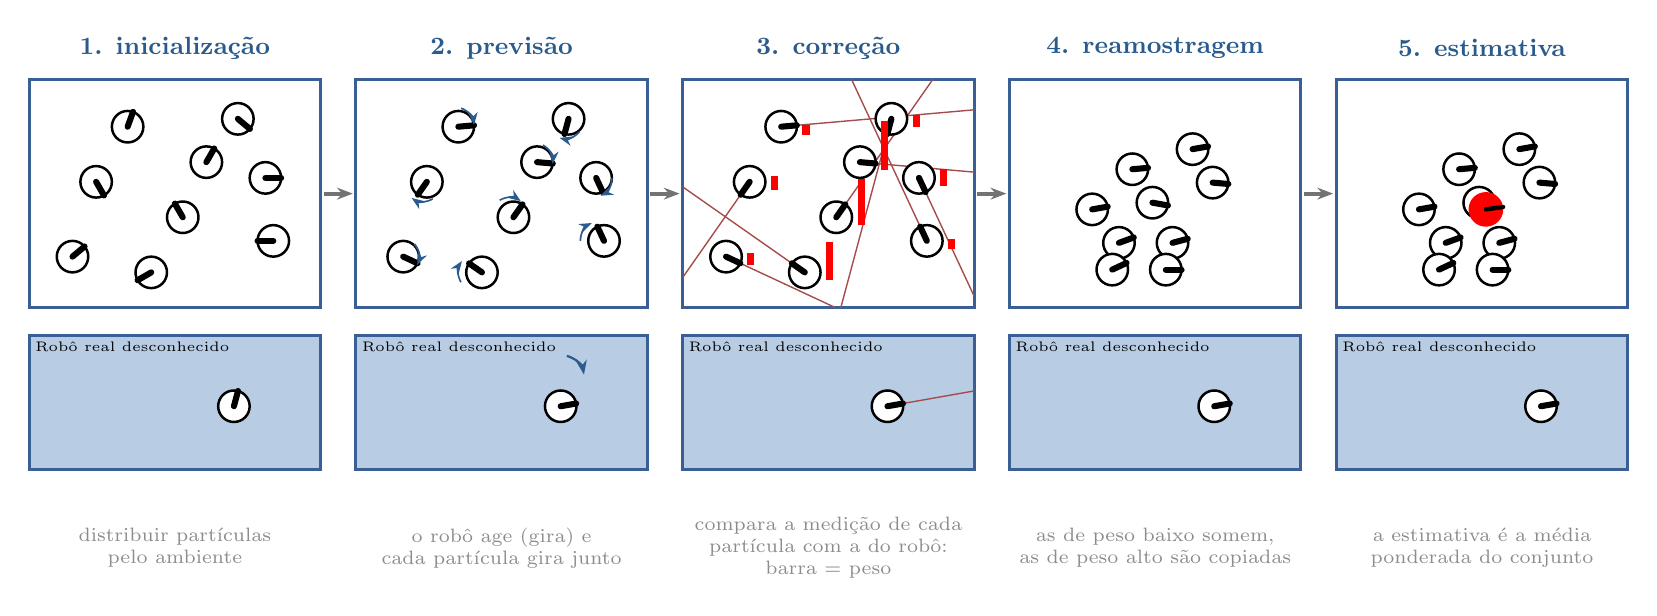
\begin{tikzpicture}[x=1cm,y=1cm]
\begin{scope}[shift={(0.00,0)}]
\node[font=\small\bfseries, dblue] at (1.85,3.30) {1. inicialização};
\draw[azulb, fill=white, line width=1.1pt] (0,0) rectangle (3.70,2.90);
\begin{scope}[shift={(0.550,0.650)}]\draw[black, fill=white, line width=0.9pt] (0,0) circle (0.20); \draw[black, line width=2.2pt, line cap=round] (0,0) -- (40:0.20); \end{scope}
\begin{scope}[shift={(1.250,2.300)}]\draw[black, fill=white, line width=0.9pt] (0,0) circle (0.20); \draw[black, line width=2.2pt, line cap=round] (0,0) -- (70:0.20); \end{scope}
\begin{scope}[shift={(1.950,1.150)}]\draw[black, fill=white, line width=0.9pt] (0,0) circle (0.20); \draw[black, line width=2.2pt, line cap=round] (0,0) -- (120:0.20); \end{scope}
\begin{scope}[shift={(2.650,2.400)}]\draw[black, fill=white, line width=0.9pt] (0,0) circle (0.20); \draw[black, line width=2.2pt, line cap=round] (0,0) -- (320:0.20); \end{scope}
\begin{scope}[shift={(3.100,0.850)}]\draw[black, fill=white, line width=0.9pt] (0,0) circle (0.20); \draw[black, line width=2.2pt, line cap=round] (0,0) -- (180:0.20); \end{scope}
\begin{scope}[shift={(0.850,1.600)}]\draw[black, fill=white, line width=0.9pt] (0,0) circle (0.20); \draw[black, line width=2.2pt, line cap=round] (0,0) -- (300:0.20); \end{scope}
\begin{scope}[shift={(2.250,1.850)}]\draw[black, fill=white, line width=0.9pt] (0,0) circle (0.20); \draw[black, line width=2.2pt, line cap=round] (0,0) -- (60:0.20); \end{scope}
\begin{scope}[shift={(1.550,0.450)}]\draw[black, fill=white, line width=0.9pt] (0,0) circle (0.20); \draw[black, line width=2.2pt, line cap=round] (0,0) -- (210:0.20); \end{scope}
\begin{scope}[shift={(3.000,1.650)}]\draw[black, fill=white, line width=0.9pt] (0,0) circle (0.20); \draw[black, line width=2.2pt, line cap=round] (0,0) -- (0:0.20); \end{scope}
\begin{scope}[shift={(0,-2.05)}]
\draw[azulb, fill=azulp, line width=1.1pt] (0,0) rectangle (3.70,1.70);
\node[font=\tiny, anchor=north west, inner sep=2pt] at (0,1.70) {Robô real desconhecido};
\begin{scope}[shift={(2.600,0.800)}]\draw[black, fill=white, line width=0.9pt] (0,0) circle (0.20); \draw[black, line width=2.2pt, line cap=round] (0,0) -- (75:0.20); \end{scope}
\end{scope}
\node[dsub, font=\scriptsize, align=center] at (1.85,-3.05) {distribuir partículas\\ pelo ambiente};
\end{scope}
\begin{scope}[shift={(4.15,0)}]
\node[font=\small\bfseries, dblue] at (1.85,3.30) {2. previsão};
\draw[azulb, fill=white, line width=1.1pt] (0,0) rectangle (3.70,2.90);
\begin{scope}[shift={(0.600,0.650)}]\draw[black, fill=white, line width=0.9pt] (0,0) circle (0.20); \draw[black, line width=2.2pt, line cap=round] (0,0) -- (-25:0.20); \end{scope}
\begin{scope}[shift={(1.300,2.300)}]\draw[black, fill=white, line width=0.9pt] (0,0) circle (0.20); \draw[black, line width=2.2pt, line cap=round] (0,0) -- (5:0.20); \end{scope}
\begin{scope}[shift={(2.000,1.150)}]\draw[black, fill=white, line width=0.9pt] (0,0) circle (0.20); \draw[black, line width=2.2pt, line cap=round] (0,0) -- (55:0.20); \end{scope}
\begin{scope}[shift={(2.700,2.400)}]\draw[black, fill=white, line width=0.9pt] (0,0) circle (0.20); \draw[black, line width=2.2pt, line cap=round] (0,0) -- (255:0.20); \end{scope}
\begin{scope}[shift={(3.150,0.850)}]\draw[black, fill=white, line width=0.9pt] (0,0) circle (0.20); \draw[black, line width=2.2pt, line cap=round] (0,0) -- (115:0.20); \end{scope}
\begin{scope}[shift={(0.900,1.600)}]\draw[black, fill=white, line width=0.9pt] (0,0) circle (0.20); \draw[black, line width=2.2pt, line cap=round] (0,0) -- (235:0.20); \end{scope}
\begin{scope}[shift={(2.300,1.850)}]\draw[black, fill=white, line width=0.9pt] (0,0) circle (0.20); \draw[black, line width=2.2pt, line cap=round] (0,0) -- (-5:0.20); \end{scope}
\begin{scope}[shift={(1.600,0.450)}]\draw[black, fill=white, line width=0.9pt] (0,0) circle (0.20); \draw[black, line width=2.2pt, line cap=round] (0,0) -- (145:0.20); \end{scope}
\begin{scope}[shift={(3.050,1.650)}]\draw[black, fill=white, line width=0.9pt] (0,0) circle (0.20); \draw[black, line width=2.2pt, line cap=round] (0,0) -- (-65:0.20); \end{scope}
\draw[dtrans, line width=0.6pt, -{Stealth[length=1.6mm]}] (0.55,0.65) ++(40:0.25) arc (40:-25:0.25);
\draw[dtrans, line width=0.6pt, -{Stealth[length=1.6mm]}] (1.25,2.30) ++(70:0.25) arc (70:5:0.25);
\draw[dtrans, line width=0.6pt, -{Stealth[length=1.6mm]}] (1.95,1.15) ++(120:0.25) arc (120:55:0.25);
\draw[dtrans, line width=0.6pt, -{Stealth[length=1.6mm]}] (2.65,2.40) ++(320:0.25) arc (320:255:0.25);
\draw[dtrans, line width=0.6pt, -{Stealth[length=1.6mm]}] (3.10,0.85) ++(180:0.25) arc (180:115:0.25);
\draw[dtrans, line width=0.6pt, -{Stealth[length=1.6mm]}] (0.85,1.60) ++(300:0.25) arc (300:235:0.25);
\draw[dtrans, line width=0.6pt, -{Stealth[length=1.6mm]}] (2.25,1.85) ++(60:0.25) arc (60:-5:0.25);
\draw[dtrans, line width=0.6pt, -{Stealth[length=1.6mm]}] (1.55,0.45) ++(210:0.25) arc (210:145:0.25);
\draw[dtrans, line width=0.6pt, -{Stealth[length=1.6mm]}] (3.00,1.65) ++(0:0.25) arc (0:-65:0.25);
\begin{scope}[shift={(0,-2.05)}]
\draw[azulb, fill=azulp, line width=1.1pt] (0,0) rectangle (3.70,1.70);
\node[font=\tiny, anchor=north west, inner sep=2pt] at (0,1.70) {Robô real desconhecido};
\begin{scope}[shift={(2.600,0.800)}]\draw[black, fill=white, line width=0.9pt] (0,0) circle (0.20); \draw[black, line width=2.2pt, line cap=round] (0,0) -- (10:0.20); \end{scope}
\end{scope}
\draw[dtrans, line width=0.8pt, -{Stealth[length=1.8mm]}] (2.6,-0.9) ++(75:0.3) arc (75:10:0.3);
\node[dsub, font=\scriptsize, align=center] at (1.85,-3.05) {o robô age (gira) e\\ cada partícula gira junto};
\end{scope}
\begin{scope}[shift={(8.30,0)}]
\node[font=\small\bfseries, dblue] at (1.85,3.30) {3. correção};
\draw[azulb, fill=white, line width=1.1pt] (0,0) rectangle (3.70,2.90);
\begin{scope}\clip (0,0) rectangle (3.70,2.90);
\draw[rayc, line width=0.5pt] (0.550,0.650) -- ++(-25:5.0);
\draw[rayc, line width=0.5pt] (1.250,2.300) -- ++(5:5.0);
\draw[rayc, line width=0.5pt] (1.950,1.150) -- ++(55:5.0);
\draw[rayc, line width=0.5pt] (2.650,2.400) -- ++(255:5.0);
\draw[rayc, line width=0.5pt] (3.100,0.850) -- ++(115:5.0);
\draw[rayc, line width=0.5pt] (0.850,1.600) -- ++(235:5.0);
\draw[rayc, line width=0.5pt] (2.250,1.850) -- ++(-5:5.0);
\draw[rayc, line width=0.5pt] (1.550,0.450) -- ++(145:5.0);
\draw[rayc, line width=0.5pt] (3.000,1.650) -- ++(-65:5.0);
\end{scope}
\begin{scope}[shift={(0.550,0.650)}]\draw[black, fill=white, line width=0.9pt] (0,0) circle (0.20); \draw[black, line width=2.2pt, line cap=round] (0,0) -- (-25:0.20); \end{scope}
\fill[red] (0.82,0.55) rectangle ++(0.09,0.14);
\begin{scope}[shift={(1.250,2.300)}]\draw[black, fill=white, line width=0.9pt] (0,0) circle (0.20); \draw[black, line width=2.2pt, line cap=round] (0,0) -- (5:0.20); \end{scope}
\fill[red] (1.52,2.20) rectangle ++(0.09,0.12);
\begin{scope}[shift={(1.950,1.150)}]\draw[black, fill=white, line width=0.9pt] (0,0) circle (0.20); \draw[black, line width=2.2pt, line cap=round] (0,0) -- (55:0.20); \end{scope}
\fill[red] (2.22,1.05) rectangle ++(0.09,0.59);
\begin{scope}[shift={(2.650,2.400)}]\draw[black, fill=white, line width=0.9pt] (0,0) circle (0.20); \draw[black, line width=2.2pt, line cap=round] (0,0) -- (255:0.20); \end{scope}
\fill[red] (2.92,2.30) rectangle ++(0.09,0.15);
\begin{scope}[shift={(3.100,0.850)}]\draw[black, fill=white, line width=0.9pt] (0,0) circle (0.20); \draw[black, line width=2.2pt, line cap=round] (0,0) -- (115:0.20); \end{scope}
\fill[red] (3.37,0.75) rectangle ++(0.09,0.12);
\begin{scope}[shift={(0.850,1.600)}]\draw[black, fill=white, line width=0.9pt] (0,0) circle (0.20); \draw[black, line width=2.2pt, line cap=round] (0,0) -- (235:0.20); \end{scope}
\fill[red] (1.12,1.50) rectangle ++(0.09,0.17);
\begin{scope}[shift={(2.250,1.850)}]\draw[black, fill=white, line width=0.9pt] (0,0) circle (0.20); \draw[black, line width=2.2pt, line cap=round] (0,0) -- (-5:0.20); \end{scope}
\fill[red] (2.52,1.75) rectangle ++(0.09,0.62);
\begin{scope}[shift={(1.550,0.450)}]\draw[black, fill=white, line width=0.9pt] (0,0) circle (0.20); \draw[black, line width=2.2pt, line cap=round] (0,0) -- (145:0.20); \end{scope}
\fill[red] (1.82,0.35) rectangle ++(0.09,0.48);
\begin{scope}[shift={(3.000,1.650)}]\draw[black, fill=white, line width=0.9pt] (0,0) circle (0.20); \draw[black, line width=2.2pt, line cap=round] (0,0) -- (-65:0.20); \end{scope}
\fill[red] (3.27,1.55) rectangle ++(0.09,0.21);
\begin{scope}[shift={(0,-2.05)}]
\draw[azulb, fill=azulp, line width=1.1pt] (0,0) rectangle (3.70,1.70);
\node[font=\tiny, anchor=north west, inner sep=2pt] at (0,1.70) {Robô real desconhecido};
\begin{scope}\clip (0,0) rectangle (3.70,1.70);\draw[rayc, line width=0.5pt] (2.600,0.800) -- ++(10:5.0);
\end{scope}
\begin{scope}[shift={(2.600,0.800)}]\draw[black, fill=white, line width=0.9pt] (0,0) circle (0.20); \draw[black, line width=2.2pt, line cap=round] (0,0) -- (10:0.20); \end{scope}
\end{scope}
\node[dsub, font=\scriptsize, align=center] at (1.85,-3.05) {compara a medição de cada\\ partícula com a do robô:\\ barra = peso};
\end{scope}
\begin{scope}[shift={(12.45,0)}]
\node[font=\small\bfseries, dblue] at (1.85,3.30) {4. reamostragem};
\draw[azulb, fill=white, line width=1.1pt] (0,0) rectangle (3.70,2.90);
\begin{scope}[shift={(1.390,0.825)}]\draw[black, fill=white, line width=0.9pt] (0,0) circle (0.20); \draw[black, line width=2.2pt, line cap=round] (0,0) -- (20:0.20); \end{scope}
\begin{scope}[shift={(1.815,1.335)}]\draw[black, fill=white, line width=0.9pt] (0,0) circle (0.20); \draw[black, line width=2.2pt, line cap=round] (0,0) -- (350:0.20); \end{scope}
\begin{scope}[shift={(1.050,1.250)}]\draw[black, fill=white, line width=0.9pt] (0,0) circle (0.20); \draw[black, line width=2.2pt, line cap=round] (0,0) -- (10:0.20); \end{scope}
\begin{scope}[shift={(2.070,0.825)}]\draw[black, fill=white, line width=0.9pt] (0,0) circle (0.20); \draw[black, line width=2.2pt, line cap=round] (0,0) -- (15:0.20); \end{scope}
\begin{scope}[shift={(1.560,1.760)}]\draw[black, fill=white, line width=0.9pt] (0,0) circle (0.20); \draw[black, line width=2.2pt, line cap=round] (0,0) -- (5:0.20); \end{scope}
\begin{scope}[shift={(2.580,1.590)}]\draw[black, fill=white, line width=0.9pt] (0,0) circle (0.20); \draw[black, line width=2.2pt, line cap=round] (0,0) -- (355:0.20); \end{scope}
\begin{scope}[shift={(2.325,2.015)}]\draw[black, fill=white, line width=0.9pt] (0,0) circle (0.20); \draw[black, line width=2.2pt, line cap=round] (0,0) -- (10:0.20); \end{scope}
\begin{scope}[shift={(1.305,0.485)}]\draw[black, fill=white, line width=0.9pt] (0,0) circle (0.20); \draw[black, line width=2.2pt, line cap=round] (0,0) -- (25:0.20); \end{scope}
\begin{scope}[shift={(1.985,0.485)}]\draw[black, fill=white, line width=0.9pt] (0,0) circle (0.20); \draw[black, line width=2.2pt, line cap=round] (0,0) -- (0:0.20); \end{scope}
\begin{scope}[shift={(0,-2.05)}]
\draw[azulb, fill=azulp, line width=1.1pt] (0,0) rectangle (3.70,1.70);
\node[font=\tiny, anchor=north west, inner sep=2pt] at (0,1.70) {Robô real desconhecido};
\begin{scope}[shift={(2.600,0.800)}]\draw[black, fill=white, line width=0.9pt] (0,0) circle (0.20); \draw[black, line width=2.2pt, line cap=round] (0,0) -- (10:0.20); \end{scope}
\end{scope}
\node[dsub, font=\scriptsize, align=center] at (1.85,-3.05) {as de peso baixo somem,\\ as de peso alto são copiadas};
\end{scope}
\begin{scope}[shift={(16.60,0)}]
\node[font=\small\bfseries, dblue] at (1.85,3.30) {5. estimativa};
\draw[azulb, fill=white, line width=1.1pt] (0,0) rectangle (3.70,2.90);
\begin{scope}[shift={(1.390,0.825)}]\draw[black, fill=white, line width=0.9pt] (0,0) circle (0.20); \draw[black, line width=2.2pt, line cap=round] (0,0) -- (20:0.20); \end{scope}
\begin{scope}[shift={(1.815,1.335)}]\draw[black, fill=white, line width=0.9pt] (0,0) circle (0.20); \draw[black, line width=2.2pt, line cap=round] (0,0) -- (350:0.20); \end{scope}
\begin{scope}[shift={(1.050,1.250)}]\draw[black, fill=white, line width=0.9pt] (0,0) circle (0.20); \draw[black, line width=2.2pt, line cap=round] (0,0) -- (10:0.20); \end{scope}
\begin{scope}[shift={(2.070,0.825)}]\draw[black, fill=white, line width=0.9pt] (0,0) circle (0.20); \draw[black, line width=2.2pt, line cap=round] (0,0) -- (15:0.20); \end{scope}
\begin{scope}[shift={(1.560,1.760)}]\draw[black, fill=white, line width=0.9pt] (0,0) circle (0.20); \draw[black, line width=2.2pt, line cap=round] (0,0) -- (5:0.20); \end{scope}
\begin{scope}[shift={(2.580,1.590)}]\draw[black, fill=white, line width=0.9pt] (0,0) circle (0.20); \draw[black, line width=2.2pt, line cap=round] (0,0) -- (355:0.20); \end{scope}
\begin{scope}[shift={(2.325,2.015)}]\draw[black, fill=white, line width=0.9pt] (0,0) circle (0.20); \draw[black, line width=2.2pt, line cap=round] (0,0) -- (10:0.20); \end{scope}
\begin{scope}[shift={(1.305,0.485)}]\draw[black, fill=white, line width=0.9pt] (0,0) circle (0.20); \draw[black, line width=2.2pt, line cap=round] (0,0) -- (25:0.20); \end{scope}
\begin{scope}[shift={(1.985,0.485)}]\draw[black, fill=white, line width=0.9pt] (0,0) circle (0.20); \draw[black, line width=2.2pt, line cap=round] (0,0) -- (0:0.20); \end{scope}
\fill[red] (1.9,1.25) circle (0.22); \draw[black, line width=1.6pt, line cap=round] (1.9,1.25) -- ++(8:0.22);
\begin{scope}[shift={(0,-2.05)}]
\draw[azulb, fill=azulp, line width=1.1pt] (0,0) rectangle (3.70,1.70);
\node[font=\tiny, anchor=north west, inner sep=2pt] at (0,1.70) {Robô real desconhecido};
\begin{scope}[shift={(2.600,0.800)}]\draw[black, fill=white, line width=0.9pt] (0,0) circle (0.20); \draw[black, line width=2.2pt, line cap=round] (0,0) -- (10:0.20); \end{scope}
\end{scope}
\node[dsub, font=\scriptsize, align=center] at (1.85,-3.05) {a estimativa é a média\\ ponderada do conjunto};
\end{scope}
\draw[->, black!55, line width=1.4pt] (3.74,1.45) -- (4.11,1.45);
\draw[->, black!55, line width=1.4pt] (7.89,1.45) -- (8.26,1.45);
\draw[->, black!55, line width=1.4pt] (12.04,1.45) -- (12.41,1.45);
\draw[->, black!55, line width=1.4pt] (16.19,1.45) -- (16.56,1.45);
\end{tikzpicture}
\end{document}
